\section{Polymorphie}
	Mithilfe von Polymorphie kann das gleiche Interface für Objekte verschiedener Typen bereitgestellt werden. Ein Bezeichner
	kann dabei Objekte unterschiedlicher Datentypen annehmen. Polymorphie wird auch Polymorphismus oder Vielgestaltigkeit
	genannt. Das Gegenteil von Polymorphie ist Monomorphie. Die meisten Codebeispiele in diesem Kapitel sind in C++
	geschrieben, da C++ alle der hier genannten Formen der Polymorphie unterstützt.
	
	Es gibt unterschiedliche Arten der Polymorphie, die man unterschiedlich einteilen kann. Eine mögliche Einteilung könnte
	beispielsweise so aussehen:
	
	\begin{table}[h]
	\begin{tabularx}{\textwidth}{$l|^X|^X}
		\rowstyle{\bfseries}  & universell                              & ad-hoc                             \\
		\rowstyle{\small}     & unendlich viele Typen                   & endliche Anzahl an Typen           \\
		\rowstyle{\small}     & eine Implementierung                    & unterschiedliche Implementierungen \\
		\hline
		\bfseries dynamisch   & \multirow{2}{*}{Inklusionspolymorphie/} &                                    \\
		\small    Laufzeit    & \multirow{2}{*}{Vererbungspolymorphie}  &                                    \\
		\small    langsamer   &                                         &                                    \\
		\hline
		\bfseries statisch    & \multirow{2}{*}{parametrische}          & \multirow{2}{*}{Überladung,}        \\
		\small    Kompilezeit & \multirow{2}{*}{Polymorphie}            & \multirow{2}{*}{Coercion}          \\
		\small    schneller   &                                         &                                    \\
	\end{tabularx}
\end{table}

	
	Polymorphie kann in statische und dynamische Polymorphie eingeteilt werden. Bei der statischen Polymorphie steht schon
	zur Kompilezeit fest, welche Funktion bzw. Methode zur Laufzeit aufgerufen werden wird. Bei der dynamischen hingegen
	wird dies erst zu Laufzeit entschieden. Welche Methode aufgerufen wird, ist abhängig vom Typen des Objekts.
	Diese Einteilung stimmt für die meisten Programmiersprachen, es gibt aber auch Ausnahmen. In dynamischen
	Programmiersprachen müssen beispielsweise alle Arten der Polymorphie dynamisch sein, da das Programm nicht kompiliert
	wird.
	Weiters kann auch zwischen universeller- und Ad-hoc-Polymorphie unterschieden werden.

	\subsection{Universelle Polymorphie}
		Mithilfe universeller Polymorphie kann das gleiche Interface für unendlich viele Typen mit nur einer einzigen Implementierung bereitgestellt werden. Diese
		Typen muss es noch gar nicht geben, sondern können auch erst in der Zukunft definiert werden. Darum wird
		universelle Polymorphie auch oft ``echte'' Vielgestaltigkeit genannt.
		
		\subsubsection{Inklusionspolymorphie}
			Inklusionspolymorphie (englisch subtyping) liegt dann vor, wenn das Liskovsche Substitutionsprinzip erfüllt ist.
			
			\paragraph{Liskovsches Substitutionsprinzip}\mbox{}\\
				Das Liskovsche Substitutionsprinzip ist erfüllt, wenn jedes Objekt von Typ A (bei Vererbung die
				Basisklasse) problemlos durch ein Objekt von Typ B (bei Vererbung die abgeleitete Klasse) ersetzt werden
				kann, ohne dass sich dabei das Verhalten ändert. Ein Objekt von Typ B muss jedoch nicht durch ein Objekt
				von Typ A ersetzt werden können. Das bedeutet, dass die Schnittstelle von Typ A eine Teilmenge der
				Schnittstelle von Typ B sein muss.
		
		\subsubsection{Vererbungspolymorphie}
			In objektorientierten Programmiersprachen wird Inklusionspolymorphie meist durch Vererbung ausgedrückt.
			Trotzdem sind Inklusionspolymorphie und Vererbungspolymorphie (englisch subclassing) nicht dasselbe, da sich
			die Vererbungspolymorphie nicht an das Liskovsche Substitutionsprinzip der halten muss. Es kann beispielsweise
			eine Methode, welche in einer in einer Basisklasse existiert, in der abgeleiteten Klasse entfernt werden. Es
			sollte aber auch bei Vererbungspolymorphie darauf geachtet werden, dass das Liskovsche Substitutionsprinzip
			eingehalten wird, auch wenn dies nicht erforderlich ist.
			
			\paragraph{Virtuelle Methoden}\mbox{}\\
				Eine virtuelle Methode, ist eine Methode bei der zur Kompilezeit noch nicht feststeht, welcher Code ausgeführt
				wird, wenn sie aufgerufen wird.
			
			\paragraph*{Beispiel -- Fahrzeuge:}\mbox{}\\
				\UseRawInputEncoding{\lstinputlisting[language={C++}]{polymorphie/universell/vererbung/beispiele/fahrzeug/fahrzeug.good.cpp}}\inputencoding{utf8}
				Eine Alternative zu Vererbungspolymorphie wäre mehrfache Auswahl (z.B. mit dem switch-Statement). Nachteil dabei
				ist, das der Code für ein Objekt nicht gesammelt an einem Platz ist, sondern über das ganze Programm verteilt.
				So müsste man immer den ganzen Code durchsuchen, wenn man z.B. einen Fahrzeugtypen hinzufügen möchte. Wenn man
				allerdings Vererbungspolymorphie verwendet, muss man lediglich eine weiter Unterklasse schreiben.
				
				\UseRawInputEncoding{\lstinputlisting[language={C++}]{polymorphie/universell/vererbung/beispiele/fahrzeug/fahrzeug.bad.cpp}}\inputencoding{utf8}
				
			
			\paragraph*{Beispiel -- Snake:}\mbox{}\\
				\begin{figure}[H]
					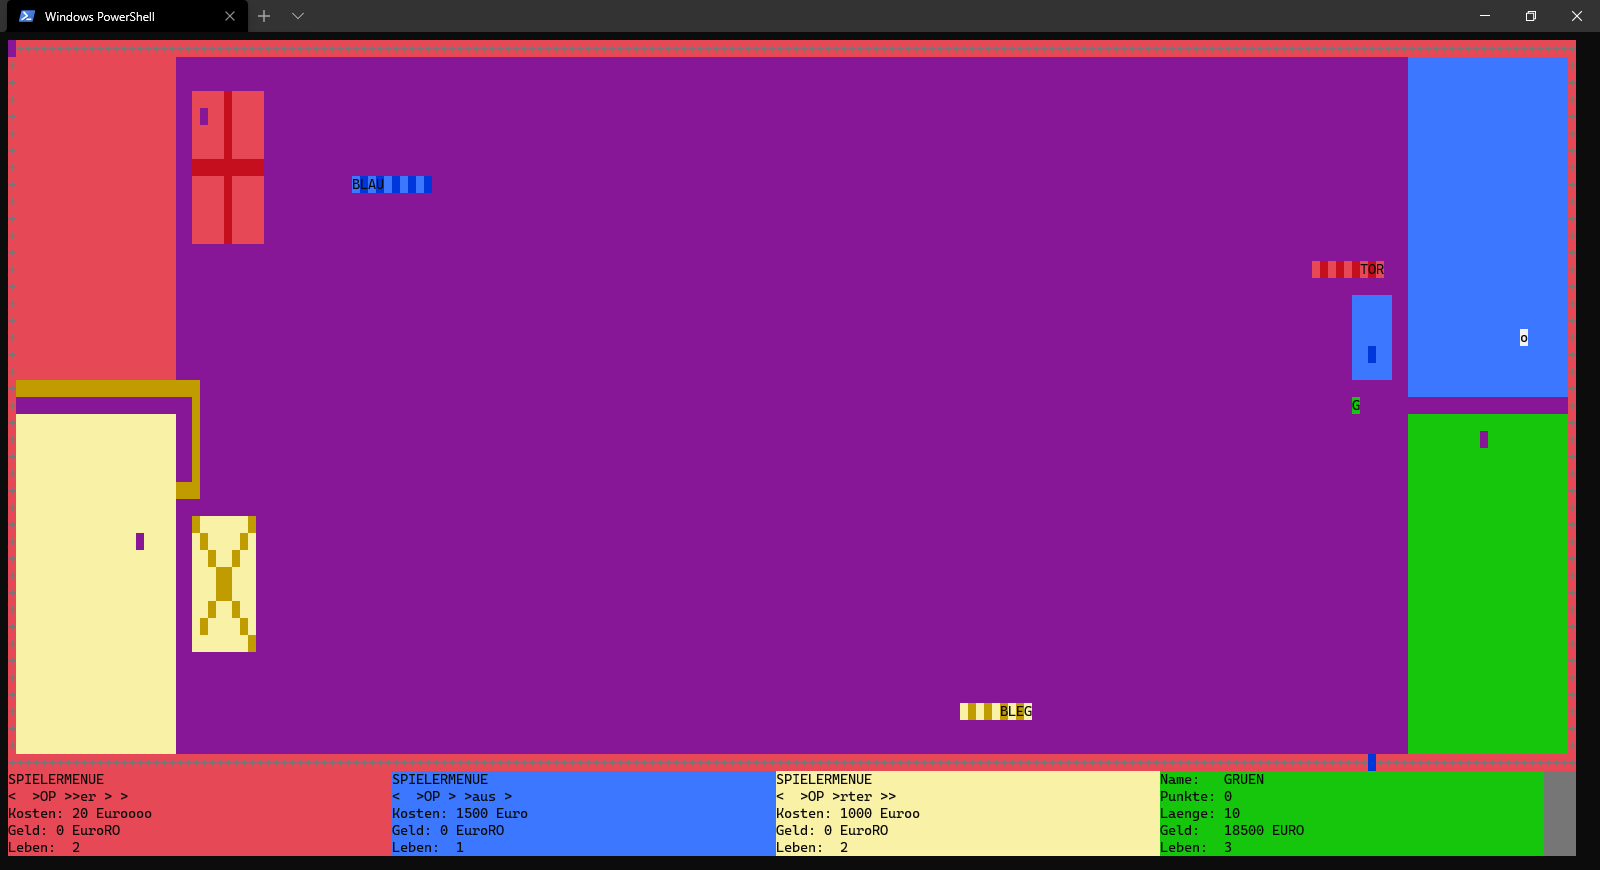
\includegraphics[width=\textwidth]{polymorphie/universell/vererbung/beispiele/snake/snake.png}
				\end{figure}
				
				Als ich in der 1. Klasse mein Multiplayer-Snake-Spiel mit ein paar Sonderregeln programmierte, kannte ich
				Klassen noch nicht. Man kann in dem Spiel unterschiedliche Arten von Gebäuden bauen (Kanonen, Mauern,
				Geldlager, Krankenhäuser, ...) und unterschiedliche Arten von Punkten fressen (normale Punkte, Geld, Leben,
				...). Dies wäre der Ideale Anwendungsfall für Vererbungspolymorphie gewesen. Da ich diese aber noch nicht
				kannte, musste ich mit mehrfacher Auswahl bzw. doppeltem Code arbeiten. Dies führte zu sehr unübersichtlichem,
				redundanten und schwer erweiterbarem Code. Jedes Mal, wenn man einen Gebäudetyp hinzufügen möchte, muss man den
				Code an unterschiedlichen Stellen im gesamten File bearbeiten.
				
				Viel Code wurde doppelt für unterschiedliche Gebäude geschrieben:
				
				\UseRawInputEncoding{\lstinputlisting[language={C++}]{polymorphie/universell/vererbung/beispiele/snake/snake_gebaeude.bad.cpp}}\inputencoding{utf8}
				
				Codeteile wie diese findet man über den gesamten Code verteilt. Abgesehen davon, dass diese
				Funktionsnamen nicht sehr aussagekräftig sind, wird das Programm durch den doppelten Code
				auch länger als notwendig. Das gesamte Programm ist 1900 Zeilen lang. Wenn man es mit
				Vererbungspolymorphie neu programmieren würde, könnte man sich mindestens die Hälfte des Codes sparen.
				Ein weiteres Problem ist, dass leicht auf ein Gebäude vergessen werden kann. Die führt zu mehr Fehlern,
				die im schlimmsten Fall gar nicht auffallen, sondern sich erst später bemerkbar machen.
				
				Mit Vererbungspolymorphie könnte eine Vererbungshierarchie beispielsweise so aussehen:
				\begin{figure}[H]
					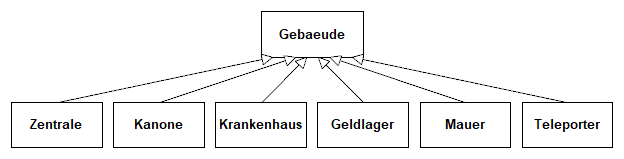
\includegraphics[width=\textwidth]{polymorphie/universell/vererbung/beispiele/snake/gebaeude.png}
				\end{figure}
				
				Die Funktionsaufrufe würden sich dadurch vereinfachen, da zur Laufzeit automatisch die richtige virtuelle
				Methode, abhängig vom Gebäudetyp, ausgewählt wird.
				\UseRawInputEncoding{\lstinputlisting[language={C++}]{polymorphie/universell/vererbung/beispiele/snake/snake_gebaeude.good.cpp}}\inputencoding{utf8}
				
				Der Vollständige Code ist auf GitHub zu finden: \url{https://github.com/PaulRaffer/Snake}
				
			\paragraph{Kreis-Ellipse-Problem}\mbox{}\\
				Das Kreis-Ellipse-Problem (bzw. Quadrat-Rechteck-Problem) ist ein Problem in der objektorientierten
				Programmierung.
				
				\subparagraph*{Problem:}\mbox{}\\
					Für eine Grafiksoftware existiert bereits die (abstrakte) Basisklasse 'Form', welche die Methoden
					'zeichnen' und 'flaeche' enthält. Einige konkrete Klassen, wie z.B. Dreieck, haben bereits von 'Form'
					geerbt. Nun sollen auch Klassen für Ellipsen und Kreise geschrieben werden, doch das ist komplizierter
					als es auf den ersten Blick scheint.
					\\\\
					Die intuitive Lösung wäre, dass die Klasse 'Kreis' von der Klasse 'Ellipse' erbt, welche wiederum von
					der Klasse 'Form' erbt, da jeder Kreis auch eine Ellipse ist und somit eine ``ist-ein''-Beziehung
					vorliegt. Zusätzlich zu den beiden Methoden 'zeichnen' und 'flaeche' implementiert die Klasse 'Ellipse'
					auch noch die Setter 'set\_x' und 'set\_y' zum skalieren der Ellipse. Diese beiden Methoden werden auch
					an die Klasse 'Kreis' weitergegeben, obwohl man bei einem Kreis nicht beide Dimensionen unabhängig
					voneinander skalieren kann. Wenn ein skalieren der einen Dimension ein automatisches skalieren der anderen
					Dimension bewirken würde, wäre das Liskovsches Substitutionsprinzip nicht erfüllt, da sich die Setter
					'set\_x' und 'set\_y' der Klasse 'Kreis' nicht gleich verhalten würden, wie die der Klasse 'Ellipse'!
					
					\begin{figure}[H]
						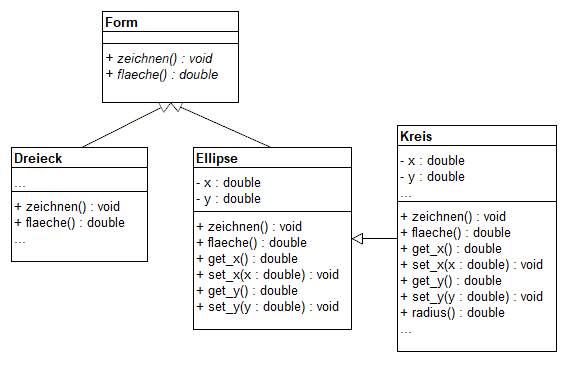
\includegraphics[scale=0.6]{polymorphie/universell/vererbung/ellipse-kreis-problem/problem.png}
					\end{figure}
				
				\subparagraph*{Lösungsvorschläge:}\mbox{}\\
					\begin{itemize}
						\item {\bfseries Fehler bei Größenänderung:}
							Bereits die Basisklasse 'Ellipse' legt fest, dass die Methoden zum ändern der Größe scheitern
							können. Dies wird z.B. durch das zurückgeben eines Fehlercodes signalisiert.
							\begin{figure}[H]
								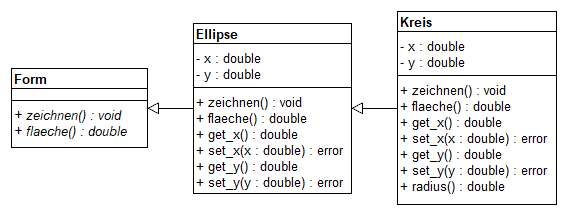
\includegraphics[scale=0.6]{polymorphie/universell/vererbung/ellipse-kreis-problem/loesungen/fehler_bei_groessenaenderung.png}
							\end{figure}
							Der Nachteil dieser Lösung ist, dass das Problem bereits auf Ebene der Basisklasse gelöst werden
							muss, und der Entwickler der Basisklasse auch alle abgeleiteten Klassen kennen muss.
							
						\item {\bfseries Ellipse erbt von Kreis:}
							Bei dieser Lösung enthält die Klasse 'Kreis' einen Setter und die entsprechende Eigenschaft. Die
							Klasse 'Ellipse' erbt bin der Klasse 'Kreis' und ergänzt den zweiten Setter und die zweite
							Eigenschaft für die zweite Dimension.
							\begin{figure}[H]
								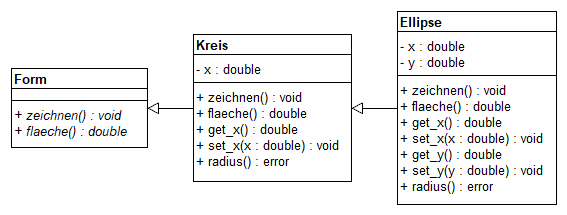
\includegraphics[scale=0.6]{polymorphie/universell/vererbung/ellipse-kreis-problem/loesungen/ellipse_erbt_von_kreis.png}
							\end{figure}
							Das Problem hierbei ist, dass die Aussage ``Jede Ellipse
							ist ein Kreis.'' nicht richtig ist, und keine ``ist-ein''-Beziehung darstellt. Es wird das
							gesamte Interface der Klasse 'Kreis' in die Klasse 'Ellipse' vererbt, auch Eigenschaften und
							Methoden, die nur ein Kreis haben sollte, wie z.B. 'radius'. Diese müssten dann entweder
							weggelassen werden oder ebenfalls einen Fehlercode zurückgeben, falls es sich um einen Ellipse
							handelt.
							
						\item {\bfseries Keine Klasse Kreis:}
							Eine weitere mögliche Lösung ist, dass es gar keine Klasse gibt, sondern die Klasse Ellipse
							eine Methode 'ist\_kreis' bereitstellt.
							\begin{figure}[H]
								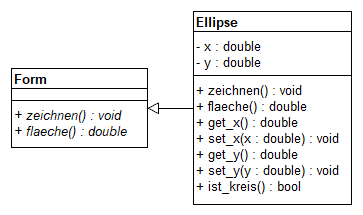
\includegraphics[scale=0.6]{polymorphie/universell/vererbung/ellipse-kreis-problem/loesungen/keine_klasse_kreis.png}
							\end{figure}
							Der Nachteil davon ist, dass der Kreis kein eigenes Interface (z.B. 'radius') bereitstellen kann.
						
						\item {\bfseries Keine Vererbungsbeziehung zwischen Ellipse und Kreis:}
							Es könnten auch beide Klassen direkt von der gemeinsamen Basisklasse 'Form' erben.
							\begin{figure}[H]
								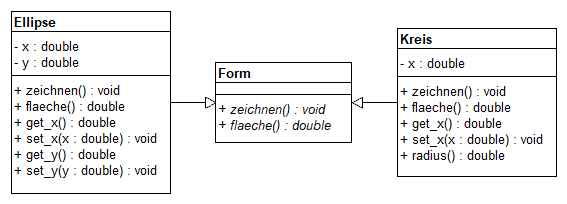
\includegraphics[scale=0.6]{polymorphie/universell/vererbung/ellipse-kreis-problem/loesungen/keine_vererbungsbeziehung_zwischen_ellipse_und_kreis.png}
							\end{figure}
							Bei diese Lösung müssten allerdings die Gemeinsamkeiten der beiden Klassen doppelt implementiert
							werden.
							
						\item {\bfseries Einführen neuer Basisklasse:}
							Man könnte auch eine weitere Klasse ('Ellipse\_oder\_kreis') einführen, welche in der Vererbungshierarchie zwischen der
							Basisklasse 'Form' und den beiden konkreten Formen 'Kreis' und 'Ellipse' steht. Diese Klasse
							könnte dann den Code enthalten, den die Klassen 'Kreis' und 'Ellipse' gemeinsam haben.
							\begin{figure}[H]
								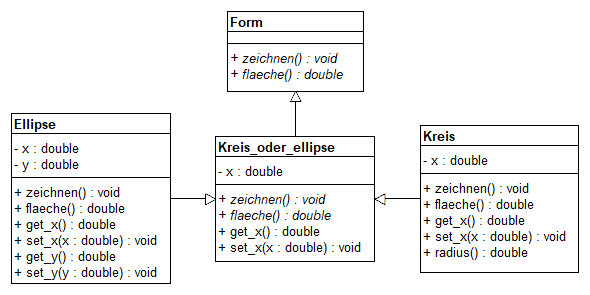
\includegraphics[scale=0.6]{polymorphie/universell/vererbung/ellipse-kreis-problem/loesungen/einfuehren_neuer_basisklasse.png}
							\end{figure}
							Der Nachteil diese Lösung ist, dass dadurch die Tiefe der Vererbungshierarchie erhöht werden würde,
							was den Code unflexibler machen würde.
					\end{itemize}
					
					Keiner der oben genannten Lösungsvorschläge ist ideal. Jeder hat seine Vor- und Nachteile.
					
					Daraus folgt, das nicht jede ``ist-ein''-Beziehung durch öffentliche Vererbung dargestellt
					werden sollte, auch wenn öffentliche Vererbung meistens ``ist-ein'' bedeuten sollte!
			
		\subsubsection{Parametrische Polymorphie}
			Parametrische Polymorphie ist vor allem in der funktionalen Programmierung weit verbreitet. Diese Art der
			Polymorphie gehört zur statischen Polymorphie, da bereits zur Kompilezeit feststeht, welche Funktion aufgerufen
			werden wird.
			TODO
			\paragraph{Einfacher parametrischen Polymorphismus}\mbox{}\\
			
			\paragraph{Beschränkter parametrischen Polymorphismus}\mbox{}\\
				Im Gegensatz zum einfachen parametrischen Polymorphismus ist der beschränkte parametrische Polymorphismus
				typensicher.
				
			\paragraph{CRTP}\mbox{}\\
				Das CRTP (Curiously recurring template pattern) kombiniert parametrische Polymorphie mit Vererbung. Hierbei
				erbt eine Klasse von einer generischen Klasse, an die die abgeleitete Klasse selbst als Typ-Parameter übergeben
				wird.
				
				\UseRawInputEncoding{\lstinputlisting[language={C++}]{polymorphie/universell/parametrisch/crtp/crtp.hpp}}\inputencoding{utf8}
				
				\subparagraph{Beispiel -- Diplomarbeit:}\mbox{}\\
				
					\begin{figure}[H]
						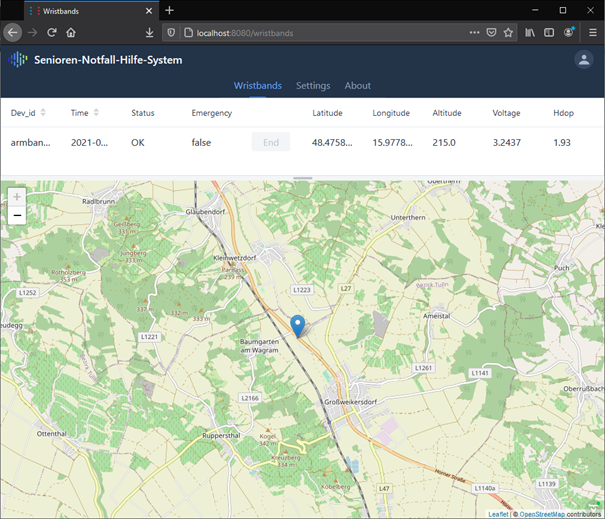
\includegraphics[width=\textwidth]{polymorphie/universell/parametrisch/crtp/beispiele/diplomarbeit/applikationsserver.png}
					\end{figure}
					
					Im Rahmen der Diplomarbeit wurde ein Senioren-Notfall-Hilfe-System entwickelt. Ein Armband nimmt Messdaten
					auf und sendet diese mittels LoRaWAN an ein Gateway. Dieses leitet die Daten an einen Server weiter,
					welcher diese darstellt. Die Position des Armbands wird auf einer Karte und zusätzlich in einer Liste
					(falls mehrere Armbänder registriert sind) angezeigt. Natürlich müssen beide Ansichten regelmäßig
					aktualisiert werden, da sich die Position oder der Status des Armbandes ändern können. Dazu wurde eine
					generische Basisklasse (UpdateView) geschrieben, welche die Logik zum aktualisieren der Daten enthält. Jede
					zweite Sekunde wird die Ansicht in einem Hintergrundthread aktualisiert. Dies geschieht durch das Aufrufen
					der Funktion 'updateFunction'. Die Funktion wird von der Unterklasse als Lambda an eine Setter-Funktion
					höherer Ordnung (setUpdateFunction) übergeben. Da es in Java keine freien Funktionen gibt muss ein
					Interface (UpdateFunction) mit einer einzigen Methode (update) erstellt werden.
					
					\UseRawInputEncoding{\lstinputlisting[language={Java}]{polymorphie/universell/parametrisch/crtp/beispiele/diplomarbeit/src/UpdateView.java}}\inputencoding{utf8}
					
					Um eine Ansicht zu erstellen, die automatisch mit neuen Daten aktualisiert wird, muss von der Klasse
					'UpdateView' geerbt werden. Dabei wird das CRTP angewandt. Daraus folgt, dass ein Objekt der Klasse MyView, wobei MyView von UpdateView<MyView> aberbt, auch ein Objekt des Typen UpdateView<MyView> sein muss. Umgekehrt ist dies streng genommen eigentlich nicht der Fall, da aber das CRTP verwendet wird und die Funktion, welche die Ansicht aktualisiert in MyView definiert wird und deshalb alle Eigenschafen und Methoden der Unterklasse (MyView selbst) kennt, ist auch eine Typumwandlung von UpdateView nach MyView problemlos (abgesehen von ein paar Warnungen) möglich.
					
					\UseRawInputEncoding{\lstinputlisting[language={Java}]{polymorphie/universell/parametrisch/crtp/beispiele/diplomarbeit/src/MapView.java}}\inputencoding{utf8}
					
					\UseRawInputEncoding{\lstinputlisting[language={Java}]{polymorphie/universell/parametrisch/crtp/beispiele/diplomarbeit/src/ListView.java}}\inputencoding{utf8}
					
	\subsection{Ad-hoc-Polymorphie}
		Mit Ad-hoc-Polymorphie kann die gleiche Schnittstelle, im Gegensatz zu universellen Polymorphie, nur für eine
		begrenzte Anzahl an bestimmten Typen bereitgestellt werden. Für jeden Typ gibt es eine eigene Implementierung
	
		\subsubsection{Coercion}
			Coercion ist eine implizite Typumwandlung vom Compiler. Diese Art der Polymorphie ist statisch, da schon zur
			Kompilezeit feststeht, welche Funktion bzw. Methode aufgerufen wird. Implizite Typumwandlungen können entweder
			zwischen zwei Variablen von eingebauten Typen, zwischen Objekten von selbst definierten Typen oder zwischen
			einer Variable eines eingebauten Typen und einem Objekt stattfinden. 
			
			\paragraph{Coercion von Variablen eingebauter Typen}\mbox{}\\
				\UseRawInputEncoding{\lstinputlisting[language={C++}]{polymorphie/adhoc/coercion/beispiele/src/eingebauteDatentypen.cpp}}\inputencoding{utf8}
				
				Ohne Coercion würde diese Zeile einen Fehler verursachen! Diese Art der Coercion ist die einzige Art der
				Polymorphie die von der Programmiersprache C unterstützt wird!
			
			\paragraph{Coercion von Objekten}\mbox{}\\
				\subparagraph*{Konvertierungskonstruktor (C++):}\mbox{}\\
					In C++ ist ein Konvertierungskonstruktor ein nicht expliziter Konstruktor der einen einzigen Parameter
					akzeptiert. Solch ein Konstruktor wandelt Objekte bzw. Variablen des Parametertyps in Objekte des
					Klassentyps um. Der Konstruktor darf nicht explizit sein, da sonst nur explizite Typumwandlungen möglich
					sind.
					
					\UseRawInputEncoding{\lstinputlisting[language={C++}]{polymorphie/adhoc/coercion/beispiele/src/konvertierungskonstruktoren.cpp}}\inputencoding{utf8}
				
				\subparagraph*{Konvertierungsoperatoren (C++):}\mbox{}\\
					In C++ werden Konvertierungsoperatoren verwendet, um ein Objekt in ein Objekt oder eine Variable eines
					anderen Typen umzuwandeln.
					
					\UseRawInputEncoding{\lstinputlisting[language={C++}]{polymorphie/adhoc/coercion/beispiele/src/konvertierungsoperatoren.cpp}}\inputencoding{utf8}
		
		\subsubsection{Überladung}
			Bei der Funktionsüberladung können verschiedene Funktionen gleich heißen und sich nur durch die Typen oder die
			Anzahl ihrer Parameter unterscheiden. Funktionen, die das gleiche Verhalten haben, sollten auch den gleichen
			Namen haben.
			
			\paragraph*{Beispiel -- Ausgabe:}
				Es sollen zwei Funktionen zur Ausgabe von einem C-String (\lstinline|char[]|) bzw. einer ganzen Zahl
				(\lstinline|int|) geschrieben werden. Da die Funktionen beide das gleiche tun, sollten sie auch den gleichen
				Namen haben.
				
				\paragraph*{C-Lösung:}
					\UseRawInputEncoding{\lstinputlisting[language={C++}]{polymorphie/adhoc/ueberladung/beispiele/print/print.c}}\inputencoding{utf8}
					\UseRawInputEncoding{\lstinputlisting[language={C++}]{polymorphie/adhoc/ueberladung/beispiele/print/print.use.c}}\inputencoding{utf8}
				
				\paragraph*{C++-Lösung:}
					\UseRawInputEncoding{\lstinputlisting[language={C++}]{polymorphie/adhoc/ueberladung/beispiele/print/print.cpp}}\inputencoding{utf8}
					\UseRawInputEncoding{\lstinputlisting[language={C++}]{polymorphie/adhoc/ueberladung/beispiele/print/print.use.cpp}}\inputencoding{utf8}
			
			\paragraph*{Beispiel -- Reset:}\mbox{}\\
				\UseRawInputEncoding{\lstinputlisting[language={C++}]{polymorphie/adhoc/ueberladung/beispiele/reset/reset.cpp}}\inputencoding{utf8}
		
			\paragraph{Operatorüberladung}\mbox{}\\
				Manche Programmiersprachen (darunter C++) ermöglichen das Überladen von Operatoren für eigene Typen. Die
				Operatorüberladung ist ein Spezialfall der Funktionsüberladung, da Operatoren auch nichts anderes als
				Funktionen mit einem oder zwei Parametern sind.
				
				Es können beispielsweise die arithmetischen Operatoren für eine eigene Bruchklasse definiert werden.
				
		\subsubsection{C++ Template-Spezialisierung}
			C++ Templates gehören eigentlich zur Kategorie der parametrischen Polymorphie, jedoch kann eine generische Funktion in C++ auch für
			bestimmte neu implementiert werden implementiert werden. Dies ist auch eine Art der Ad-hoc-Polymorphie.
			
	\subsection{Kombination verschiedener Arten der Polymorphie}\mbox{}\\
		Verschiedene Arten der Polymorphie können meist sehr gut in einem Projekt kombiniert werden.
		\subsubsection*{Beispiel -- Bruchklasse:}
			In meiner Bruchklassen (\url{https://github.com/PaulRaffer/raffer_cpplib-fraction/blob/cpp14/fraction.hpp}) habe ich z.B. die
			drei wichtigsten Arten der statischen Polymorphie (parametrische Polymorphie, Coercion und Überladung) verwendet.
			
			Parametrische Polymorphie wird verwendet, um beliebige Zähler bzw. Nenner beliebiger Typen zuzulassen. So können beispielsweise
			Doppelbrüche (\lstinline|fraction<fraction<int>, fraction<int>>|) oder Brüche mit komplexen Zahlen als Zähler bzw. Nenner (\lstinline|fraction<complex<double>, complex<double>>|) erstellt
			werden.
			
			Des weiteren hat das Klassen-Template einen Konvertierungskonstruktor, der Objekte des Zähler-Typen implizit in Brüche
			umwandeln kann.
			
			Mit Brüchen kann auch gerechnet werden, da die arithmetischen Operatoren überladen wurden.